%!TEX root = ../agi_mfws414ali.tex
\section{Dokumentation des AntMe!-Projektes}
\label{doku}

Im folgenden Kapitel wird die im Rahmen der des AntMe!-Projektes umgesetzte Strategie zunächst grundlegend beschrieben, bevor die Strategieentscheidungen im Einzelnen erläutert und begründet werden. Schließlich werden diverse Messreihen herangezogen, um die erreichten Punktzahlen hinsichtlich der Anforderung an die Höhe bewerten zu können.

\subsection{Strategie}
Dieser Abschnitt erläutert die Strategie zunächst im Überblick, bevor die Umsetzung der Strategie im Detail behandelt wird. Die verschiedenen Domänen von AntMe!, wie die Fortbewegung oder der Kampf werden dabei einzeln betrachtet und die Stellen, wo diese in einander übergreifen, aufgezeigt. Als erstes wird erklärt, wie die Kasten realisiert wurden, gefolgt von den Grundfunktionalitäten der Fortbewegung, der Kommunikation und des Ticks. Sind die elementaren Konzepte der Strategie erklärt, wird das Verhalten der Ameisen im Hinblick auf die Nahrung und den Kampf dargelegt.

\subsubsection{Überblick} \label{ssec:overview}
Der grundlegende Fokus der vorliegenden Strategie liegt auf dem Kampf gegen Wanzen und feindliche Ameisen, die Spezialisierung der Ameisen ist entsprechend daraufhin ausgerichtet. Dennoch ist das Sammeln von Nahrung ein essentieller Bestandteil der Strategie. Aus taktischen Gründen hinsichtlich der Nahrungssuche ist das Ameisenvolk in zwei Kasten aufgeteilt. Die Kasten unterscheiden sich einzig durch das Verhalten, die Spezialisierungen sind hingegen identisch. Dabei ist die eine Kaste stärker auf das Sammeln von Zucker ausgerichtet als die andere.

Die Spezialisierung auf den Kampf ist ein Kompromiss, da das Ameisenvolk sowohl im Einspieler-Modus als auch im Mehrspieler-Modus erfolgreich sein soll. Im Einzelspiel sind durch die Fokussierung auf die Nahrungssammlung i.d.R. höhere Punktzahlen erzielbar. Eine solche Strategie ist im Mehrspieler jedoch nur begrenzt tauglich. Einerseits kommt es zu erheblichen Problemen, wenn das gegnerische Ameisenvolk auf den Kampf gegen Ameisen ausgelegt ist. Anderseits kann dies in bestimmten Fällen ebenfalls nachteilig sein, wenn der Gegenspieler gleicherweise ausschließlich Nahrung sammelt. Da das Spielfeld jede Runde erneut zufällig aufgebaut wird, kann es vorkommen, dass der Gegner näher an der Nahrung gelegen ist. Dadurch, dass die eigenen Ameisen weitere Wege zurücklegen müssen, um die Nahrung einzusammeln, ist eine Niederlage in diesen Situationen unausweichlich. Die Entscheidung über Sieg oder Niederlage ist in der Konstellation also relativ willkürlich, vorausgesetzt die feindlichen Ameisen sind etwa gleich stark im Sammeln. Im Umkehrschluss bedeutet dies, dass die Kampf-Spezialisierung entscheidend im Mehrspieler ist. Zum einen sind die Ameisen so in der Lage sich gegen feindliche Ameisen zu verteidigen. Des Weiteren sind sie klar im Vorteil gegenüber Ameisen, die nicht im Kampf spezialisiert sind. 

\subsubsection{Kasten}
Das Ameisenvolk \textit{LipkeAnts} wurde in zwei Kasten unterteilt. Die Kaste \textit{NormalAnt} ist die Standardkaste, also die mit dem größten Bevölkerungsanteil. Zusätzlich gibt es die Kaste \textit{SugarAnt}, welche einen stärkeren Fokus auf dem Sammeln von Zucker hat.

\subheading{Spezialisierungen}

Eine Ameise in AntMe! besitzt bestimmte Fähigkeiten bzw. Eigenschaften\footnote{In AntMe! wird von Fähigkeiten gesprochen, da es sich bei bereits Eigenschaften um ein Sprachkonstrukt in den Programmiersprachen C\# und Visual Basic handelt.}, wie bspw. die Bewegungsgeschwindigkeit, die Lebenspunkte und weitere. Jede Fähigkeit kann verbessert oder verschlechtert werden, jedoch müssen die Fähigkeiten insgesamt ausgeglichen sein, dies wird Spezialisierung genannt\footcite{AntMeWiki1}.

Den Fähigkeiten können Punkte im Wertebereich von -1 bis +2 vergeben werden. Dabei muss die Summe aller Fähigkeitswerte <= 0 sein, sodass keine ungerechte Verteilung möglich ist und die Spezialisierung gut durchdacht sein muss. Standardmäßig sind alle Fähigkeiten gleich null gesetzt (siehe Tabelle ~\ref{tab:standardProps}).

\begin{table}[hbt]
\centering
\begin{minipage}[t]{.7\textwidth} % Breite der Tabelle		
\caption{Fähigkeiten ohne Spezialisierung (Standard)} % Überschrift
\begin{tabularx}{\columnwidth}{rXr}
\toprule
Fähigkeit & Beschreibung & Wert\\
\midrule
Geschwindigkeit & Schritte pro Runde & 4\\
Drehgeschwindigkeit & Grad pro Runde & 8\\
Last & Einheiten Nahrung & 5\\
Sichtweite & Schritte & 60\\
Reichweite & Schritte & 2250\\
Energie & Lebenspunkte & 100\\
Angriff & Lebenspunkte pro Runde & 10\\
\bottomrule
\end{tabularx}
\source{Eigene Darstellung in Anlehnung an \cite{AntMeWiki3}} % Quelle
\label{tab:standardProps}
\end{minipage}
\end{table}

Die Kasten \textit{NormalAnt} und \textit{SugarAnt} des Ameisenvolkes \textit{LipkeAnts} haben beide die gleiche Spezialisierung (siehe Tabelle \ref{tab:lipkeAntsProps}). Dies hat den Grund, dass die Ausrichtung auf den Kampf ein wichtiger Bestandteil der Strategie darstellt, um im Mehrspieler-Modus zu bestehen. Zwar wäre es eine Möglichkeit auf die Gegebenheiten des aktuellen Spieles zu reagieren, indem nur noch Ameisen geboren werden die gegen die feindlichen Ameisen effektiv sind. Diese dynamische Anpassung während der Laufzeit ist jedoch nicht möglich, da es sich bei den \textit{LipkeAnts} um nicht-statische Ameisen handelt. Statische Ameisen verfügen über die Möglichkeit ein globales Gehirn, in Form von statischen Variablen, auf die jede Ameise zugreifen kann, nachzubilden. Bei nicht-statischen Ameisen ist zwar auch eine Kommunikation über Duftmarken möglich (siehe \ref{sssec:communication}), auf diese kann aber erst reagiert werden, wenn die Ameise bereits geboren ist.

\begin{table}[hbt]
\centering
\begin{minipage}[t]{.6\textwidth} % Breite der Tabelle		
\caption{Spezialisierung \textit{LipkeAnts}} % Überschrift
\begin{tabularx}{\columnwidth}{rXr}
\toprule
Fähigkeit & Punkte & Wert\\
\midrule
Geschwindigkeit & 0 & 4\\
Drehgeschwindigkeit & -1 & 6\\
Last & -1 & 4\\
Sichtweite & -1 & 45\\
Reichweite & -1 & 1800\\
Energie & 2 & 250\\
Angriff & 2 & 30\\
\bottomrule
\end{tabularx}
\source{Eigene Darstellung in Anlehnung an \cite{AntMeWiki3}} % Quelle
\label{tab:lipkeAntsProps}
\end{minipage}
\end{table}

Bei der Spezialisierung der \textit{LipkeAnts} wurde für die Fähigkeiten Angriff und Energie die maximale Punktzahl vergeben. Die Ameisen sind somit im Vorteil gegen im Kampf gegen die meisten Spezialisierungen anderer Völker, einzig Ameisenvölker, die ebenfalls jeweils zwei Punkte auf Angriff und Energie gesetzt haben sind in der Lage gegen die \textit{LipkeAnts} zu bestehen. Im Falle von gleich starken Ameisen gehen die Kämpfe meistens unentschieden aus (beide Ameisen sterben bei dem Kampf), höchstens wenn eine der Ameisen bereits geschwächt in den Kampf geht verliert diese. Oder aber wenn eine der Ameisen zuerst angreift, da die andere vorher z.B. mit dem Tragen eines Apfels beschäftigt war. Weiterhin wurden die Fähigkeiten Drehgeschwindigkeit, Last, Sichtweite und Reichweite auf den Minimalwert gesetzt. Diese Fähigkeiten sind bei einer Ausrichtung auf den Kampf vernachlässigbar. Zudem ist aufgrund der Regeln für die Spezialisierung nur ein Punkt übrig, wenn zwei andere Werte bereits auf zwei gesetzt sind. Von den fünf restlichen Fähigkeiten ist die Geschwindigkeit neben der Energie und dem Angriff die wichtigste für die hier verfolgte Strategie und wurde daher auf null, also den Standardwert gesetzt. Die Geschwindigkeit ist wichtig, weil die Ameisen so schneller Nahrung befördern können. Auch im Kampf ist die Geschwindigkeit nicht zu vernachlässigen, da Ameisen, die die Geschwindigkeit auf minus eins gesetzt haben zu langsam sind, um eine Wanze einzuholen oder gegnerische Ameisen zu verfolgen.

\subheading{Bestimmung der Kaste}

Jedes Mal, wenn eine Ameise geboren wird, muss dieser Ameise eine Kaste zugewiesen werden. Zu diesem Zweck wird die Methode \textit{ChooseCaste} verwendet. Innerhalb dieser Methode kann auf die aktuelle Anzahl an Ameisen in den jeweiligen Kasten zugegriffen werden. Im Falle der \textit{LipkeAnts} wird mit \textit{ChooseCaste} der Anteil der Kaste \textit{NormalAnt} auf 75 Prozent bzw. bei der Kaste \textit{SugarAnt} auf 25 Prozent reguliert.

\subheading{Verhalten}

Wie bereits erwähnt, unterscheidet sich das Verhalten der Kasten \textit{NormalAnt} und \textit{SugarAnt}. Im Wesentlichen handelt es sich dabei um die Fortbewegung, den Umgang mit Zucker sowie das Verhalten bei Wanzen. Ameisen der Kaste \textit{SugarAnt} passen zudem ihr Verhalten dynamisch an die gegebene Situation an. Wird eine Ameise aus dieser Kaste neu geboren, so setzt diese einen stärkeren Fokus auf den Zucker als die Ameisen der Kaste \textit{NormalAnt}. Sobald jedoch erkannt wird, dass feindliche Ameisen im Spiel sind, ändert die Ameise der Kaste \textit{SugarAnt} ihr Verhalten, um sich von diesem Zeitpunkt an wie eine Ameise der Kaste \textit{NormalAnt} zu verhalten. Die Unterschiede in diesen Verhaltenspunkten werden in den folgenden Abschnitten genauer betrachtet.

\subsubsection{Fortbewegung}
Die Fortbewegung der Ameisen in AntMe! wird mithilfe dem Konzept der Zustandsmaschine realisiert. Eine Ameise kann sich in den Zuständen \textit{Warten}, \textit{Drehen}, \textit{Gehen} und \textit{Ziel verfolgen} befinden (siehe Abbildung \ref{img:states}). Der Ausgangszustand einer Ameise ist \textit{Warten}, der Wechsel eines Zustandes in den nächsten kann explizit durch Befehle wie \textit{GoForward} oder implizit durch bestimmte Ereignisse hervorgerufen werden.\footcite[Vgl.][]{AntMeWiki2}

\begin{figure}[hbt]
\centering
\begin{minipage}[t]{0.5\textwidth} % Breite, z.B. 1\textwidth		
\caption{Statusablauf einer Ameise} % Überschrift
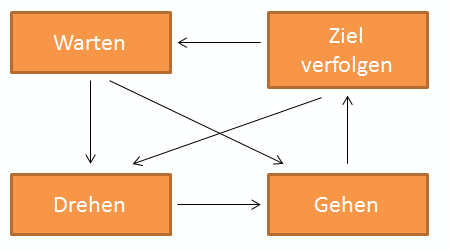
\includegraphics[width=1\textwidth]{img/AntStates.png}\\ % Pfad
\source{\cite{AntMeWiki2}} % Quelle
\label{img:states}
\end{minipage}
\end{figure}

\subheading{Wartet}

Befindet sich eine Ameise im Zustand \textit{Warten}, hat diese weder ein Ziel noch den Befehl eine bestimmte Strecke zu gehen oder sich zu drehen, sodass die Ameise still steht und auf weitere Befehle wartet. Jede Runde wird das Ereignis \textit{Waiting} aufgerufen, dieses Ereignis stellt die zentrale Steuerung der Fortbewegung dar. Aus strategischen Gründen sollen sich die Ameisen der Kasten \textit{NormalAnt} und \textit{SugarAnt} unterschiedlich bewegen. \textit{NormalAnt}-Ameisen sollen zunächst 40 Schritte gerade aus laufen und im Anschluss eine Drehung um einen zufälligen Wert zwischen -10 und +10 ausführen. Dies hat zur Folge, dass die Ameisen relativ verstreut über das Spielfeld laufen und somit in der Lage sind eine größere Fläche abzusuchen. Die erweiterten Suchbereiche der Ameisen führen zu einer höheren Wahrscheinlichkeit, dass sie auf einen Apfel, eine Wanze oder weitere Spielelemente trifft. Die \textit{SugarAnt}-Ameisen zwar ebenfalls einen Richtungswechsel vornehmen, jedoch erst nach 150 Schritten, da diese eine Spur zum Zucker suchen sollen. Wenn in der aktuellen Richtung nach 150 Schritten keine Spur zu finden ist, sollen die Ameisen sich um einen zufälligen Winkel zwischen -15 Grad bis +15 Grad drehen. Der Winkel ist größer gewählt, da die Zuckerhaufen teils recht weiträumig über das Spielfeld verteilt sind. Ist eine \textit{SugarAnt}-Ameise allerdings in Kenntnis darüber, dass feindliche Ameisen existieren, soll diese sich wie eine \textit{NormalAnt}-Ameise verhalten.

\subheading{Tick}

Neben dem Wartet-Ereignis ist das Tick-Ereignis eines der wichtigsten Ereignisse für die Bewegungssteuerung der Ameisen. Da im Tick-Ereignis jedoch noch weitere Aktionen abgearbeitet werden, wird dieses in einem gesonderten Abschnitt behandelt (siehe \ref{sssec:tick}).

\subheading{Wird müde}

Sobald die restliche Strecke einer Ameise ein Drittel der verfügbaren Schritte erreicht hat wird das Ereignis \textit{GettingTired} aufgerufen. Zu diesem Zeitpunkt könnte man der Ameise befehlen zum Ameisenbau zurückzukehren, damit diese nicht verhungert. Denn wenn eine Ameise die maximale Reichweite erreicht hat, stirbt diese am Hungertod. Dies wirkt sich i.d.R. nachteilig auf die Endpunktzahl aus, da die Ameise nicht optimal eingesetzt wurde. Wenn eine Ameise bspw. zum Todeszeitpunkt ein Zucker zum Bau transportiert, lässt es diesen fallen. Zucker der fallen gelassen wird ist verloren und kann nicht mehr von anderen Ameisen aufgesammelt werden. Diese Ameise hat in einer Zeitspanne, in der eine Ameise mit genügend Reststrecke Punkte erzielt hätte keine Punkte erzielt und somit Zeit verschwendet. 

Nach einigen Testläufen hat sich jedoch herausgestellt, dass die ein Drittel Marke oftmals nicht ausreichend war, um den Hungertod zu verhindern. Weiterhin kann es sein, dass der Bau relativ weit mittig gelegen ist, sodass die Ameise bei einem Drittel Reststrecke zum Bau zurückkehrt, obwohl die Distanz zum Ameisenhügel weniger als diese Reststrecke beträgt. Aus diesem Grund wurde auf den Gebrauch dieses Ereignisses verzichtet und ein eigener Mechanismus innerhalb des Tick-Ereignisses realisiert, der bezweckt, dass die Ameisen rechtzeitig zum Bau zurückkehren (siehe \ref{sssec:tick}).

\subheading{Ist gestorben}

Ein weiteres Ereignis, welches zu den Ereignissen der Fortbewegung zählt, ist der Todeszeitpunkt, denn der Tod wird als letzte Bewegung der Ameise gezählt. Ist eine Ameise gestorben, kann diese keine weiteren Aktionen ausführen. Da es sich bei dem Volk \textit{LipkeAnts} jedoch um nicht-statische Ameisen handelt, findet das Ereignis \textit{HasDied} keine Anwendungsfälle. Demgegenüber sind statische Ameisen in der Lage die Todesart im globalen Gedächtnis (statische Variablen) zu hinterlegen, sodass die anderen Ameisen darauf reagieren können. Mögliche Anwendungsfälle wäre bspw. das Zählen der aufgetretenen Todesarten, sodass bei der Bestimmung der Kaste nur noch Kasten ausgewählt werden, die eine Antwort auf eine übermäßige Todeszahl einer bestimmten Todesart darstellen.

\subsubsection{Kommunikation} \label{sssec:communication}
Die Kommunikation zwischen den Ameisen ist ein zentraler Mechanismus, ohne den ein erfolgreiches Ameisenvolk nicht realisierbar ist. In dem Großteil der den Ameisen zur Verfügung stehenden Ereignisse wird die Kommunikation verwendet. 

Ameisen sind in der Lage Duftmarken abzusetzen und diese Markierungen mit Informationen anzureichern. Andere Ameisen aus dem eigenen Volk können diese Duftmarken riechen und die Informationen daraus auslesen. Es besteht zudem die Möglichkeit, die Größe der Markierung festzulegen. Die Größe hat Einfluss auf die Dauer, für die eine Duftmarke bestehen bleibt. Diese beiden Faktoren sind wichtig, um die Anzahl an Ameisen, die auf die Markierung aufmerksam werden, zu regulieren. Je größer die Duftmarke, desto mehr Ameisen können diese wahrnehmen, allerdings löst sie sich auch schneller wieder auf. Daher ist die richtige Größe oft entscheidend und ermöglicht unterschiedlichste Taktiken. Besonders nicht-statische Ameisen, wie die \textit{LipkeAnts} sind stark von der Kommunikation über Duftmarken abhängig. Es können nur die Duftmarken der Ameisen aus dem eigenen Volk erkannt werden.

Bei den Informationen, die über eine Duftmarke übermittelt werden können, handelt es sich lediglich um einen 32 Bit Integer-Wert. Die hieraus resultierenden Möglichkeiten sind somit standardmäßig sehr begrenzt. Für simple Strategien reicht das i.d.R. aus, da dort oft nur die Richtung in der sich ein Spielelement (Nahrung, Gegner) befindet übergeben wird. Dabei handelt es sich um gleichartige Informationen. Die in dieser Strategie verfolgten Ansätze erfordern jedoch neben der eigentlichen Information zusätzlich die Möglichkeit die Art der Information zu unterscheiden, um divergente Informationen zu übertragen. Zu diesem Zweck wurde die Methode \textit{CreateMarkerInformation} (siehe Listing \ref{list:createMarkerInformation}) entworfen. Dieser Methode werden die Information sowie der Typ der Information übergeben. Der Informationstyp ist wie die Information auch ein Integer-Wert, jedoch kann die Information verschieden lang sein, wohingegen der Informationstyp auf eine einstellige Zahl festgelegt wurde (als Klassen-Member definiert). Es wird zwischen folgenden Informationstypen unterschieden:
\begin{compactitem}
   \item Es wurde ein Apfel gesehen
   \item Es wurde ein Zuckerhaufen gesehen
   \item Es wurde eine Wanze gesehen
   \item Es wurde eine feindliche Ameise gesehen
\end{compactitem}

\begin{figure}[bht]
\begin{lstlisting}[caption=Methode zum Erstellen verbesserter Marker-Informationen, label=list:createMarkerInformation]
private int CreateMarkerInformation(int information, int infoType)
{
    string _infoType = infoType.ToString();
    string _information = information.ToString().PadLeft(4, '0');
    string advancedInformation = _infoType + _information;

    return Convert.ToInt32(advancedInformation);
}
\end{lstlisting}
\end{figure}

\textit{CreateMarkerInformation} wandelt die beiden Integer-Werte zunächst in einen String,  damit diese aneinandergefügt werden können, bevor sie wieder in einen Integer konvertiert werden. Dies ist notwendig, um einerseits die Information mit führenden Nullen aufzufüllen, da die Informationen unterschiedlich lang sind. Des Weiteren kann so die spätere Extraktion erleichtert werden, denn die zuvor zusammengefügten Strings müssen später lediglich wieder getrennt werden. Für die Extraktion wurde die Hilfsklasse \textit{MarkerInformation} entwickelt, welche eine zielführende Datenhaltung realisiert (siehe Listing \ref{list:markerInformation}).

\begin{figure}[bht]
\begin{lstlisting}[caption=Hilfsklasse zum Extrahieren der verbesserten Marker-Informationen, label=list:markerInformation]
public class MarkerInformation
{
    public MarkerInformation(int information)
    {
        string info = information.ToString();
        this.Data = Convert.ToInt32(info.Substring(1));
        this.InfoType = Convert.ToInt32(info.Substring(0, 1));
    }

    public int Data { get; set; }

    public int InfoType { get; set; }
}
\end{lstlisting}
\end{figure}

Wenn eine Ameise die Duftmarke einer anderen Ameise riecht, kann sie auf die über die Markierung übermittelte Information zugreifen. Im Falle der \textit{LipkeAnts} muss diese Information zuerst noch mithilfe der Klasse \textit{MarkerInformation} in Hauptinformation und Informationstyp zerlegt werden. Anhand des Informationstyps wird dann entschieden, wie mit der Information verfahren werden soll. Wurde über die Duftmarke mitgeteilt, dass sich andere Ameisenvölker im Spiel befinden, merkt sich die Ameise diese Information, damit sie das Verhalten dementsprechend anpassen kann. Handelt es sich um eine Apfel-, Zucker- oder Wanzen-Markierung, werden der Ameise jeweils zielführende Befehle erteilt.

\subheading{Apfel-Markierung}

Vorausgesetzt die Ameise trägt zur Zeit keinen Apfel oder Zucker, hat kein Ziel und die Anzahl an Ameisen aus dem eigenen Volk im 360 Grad Sichtfeld ist geringer als die Anzahl an benötigten Träger für den Apfel, soll die Ameise zum Mittelpunkt der Duftmarke gehen. Es wird darauf gesetzt, dass die Ameise entweder den Apfel entdeckt oder eine weitere Markierung auffindet, sobald sie in der Mitte der Duftmarke angekommen ist. Die Anzahl der Träger, die für den Apfel notwendig sind wird als Information über die Duftmarke übermittelt. Andernfalls soll die Ameise stoppen, wodurch sie das Ziel verliert und sich auf andere Aufgaben konzentrieren kann.

\subheading{Zucker-Markierung}

Bei einer Zucker-Markierung soll wie auch bei der Apfel-Markierung überprüft werden, dass die Ameise weder Last noch Ziel hat. Zusätzlich sollen nur \textit{SugarAnt}-Ameisen auf die Markierung reagieren. Zuletzt wird abgefragt, ob die über die Duftmarke übertragene Richtung des Zuckers eine andere ist, als die aktuelle Richtung der Ameise. Denn wenn alle Abfragen zutreffend sind, soll die Ameise sich in die Richtung des Zuckers drehen und 150 Schritte geradeaus laufen, da die Spur zum Zucker eventuell nicht präzise genug ist, um die Ameise zielsicher zum Zucker zu führen. Deswegen soll die Ameise eine längere Strecke gerade aus laufen um dem vorzubeugen. Für eine stabile Zuckerstraße ist der Anteil der \textit{SugarAnt}-Ameisen mit 25 Prozent zu gering.

\subheading{Wanzen-Markierung}

Wird eine Wanzen-Markierung entdeckt wird als erstes geprüft, ob sich weniger als acht Ameisen aus dem eigenen Volk in der Nähe befinden. Sind es mehr wird die Markierung ignoriert, weil nur eine begrenzte Anzahl an Ameisen für das Besiegen einer Wanze notwendig sind. Zusätzlich muss eine von folgenden vier Bedingungen zutreffen, damit die Ameise auf die Duftmarke reagiert:
\begin{compactitem}
   \item Die Ameise hat kein Ziel,
   \item \textbf{oder} die Ameise hat keine Wanze zum Ziel \textbf{und} trägt keinen Apfel,
   \item \textbf{oder} es handelt sich um eine \textit{NormalAnt}-Ameise \textbf{und} sie befördert Zucker,
   \item \textbf{oder} es handelt sich um eine \textit{SugarAnt}-Ameise, die sich wie eine normale Ameise  verhalten soll \textbf{und} sie befördert Zucker.
\end{compactitem}

Die Zusatzbedingungen bilden also zahlreiche Fälle ab, in denen die Ameise auf die Duftmarke reagieren soll. So soll sie die Markierung ignorieren, wenn sie einen Apfel trägt, aber wahrnehmen, wenn sie Zucker trägt (verallgemeinert), denn Wanzen und auch Äpfel bringen aufgrund der Spezialisierung auf Kampf mehr Punkte ein, als Zucker. Auch wenn die Ameise auf dem Weg zu einer feindlichen Ameise oder einem Marker ist, soll sie die Wanzen-Markierung wahrnehmen, da Wanzen Priorität haben. Zudem soll die Ameise nicht abgelenkt werden, wenn sie bereits einer Wanze folgt. Ist eine Kombination zutreffend, soll die Ameise den Zucker fallen lassen, falls sie welchen trägt und in die Mitte der Markierung laufen.

Über die Möglichkeit Duftmarken zu riechen hinaus, existieren zudem Ereignisse, die ausgelöst werden, wenn eine Ameise aus dem eigenen Volk bzw. aus der eigenen Kaste gesehen wurden (\textit{SpotsFriend}, \textit{SpotsTeammate}). Diese können dazu genutzt werden, um gezielt mit den Ameisen im eigenen Umkreis zu kommunizieren. In der hier vorgestellten Strategie werden diese jedoch nicht verwendet. Dies hat den Grund, dass bereits für alle wichtigen Informationen entsprechende Duftmarken erstellt werden, wie z.B. \gqq{In Richtung x befindet sich Zucker!}, \gqq{Es gibt einen Apfel in der Nähe der noch Träger braucht!}. Mögliche Anwendungsfälle wären beispielsweise die Übermittlung von Informationen zwischen den Ameisen, wie \gqq{Ich trage einen Apfel, hilf mir!}. Darüber hinaus könnten diese Ereignisse dazu genutzt werden die Bildung von Gruppen zu koordinieren, allerdings sieht diese Strategie keine Gruppenbildung vor. Und Informationen über die Spielelemente (Äpfel, Zucker, ...) werden bereits auf eine effektivere Art kommuniziert. Weil eine Ameise nahezu dauerhaft von befreundeten Ameisen umgeben ist, werden die Ereignisse viel zu oft aufgerufen, wodurch die Markierungen sich überlagern und nicht mehr präzise sind, die Ameisen würden durch den vielen Input zu sehr abgelenkt.

\subsubsection{Tick} \label{sssec:tick}
Das \textit{Tick}-Ereignis wird ohne Ausnahme in jeder Runde aufgerufen, dies ermöglicht eine präzise Steuerung der Ameisen sowie die Realisierung zahlreicher taktischer Konzepte. Bei den \textit{LipkeAnts} wird im \textit{Tick} zwischen dem Setzen von Parametern und dem Ausführen von Aktionen unterschieden.

Innerhalb des Ereignisses \textit{Tick} wird der Parameter \textit{HasSeenForeignAnt} auf \textit{false} gesetzt, wenn basierend auf verschiedenen Anhaltspunkten davon ausgegangen werden kann, dass keine feindlichen Ameisen existieren. Dies trifft zu, wenn die Ameise bereits mehr als 200 Schritte gelaufen ist, zu dem Geburtszeitpunkt bereits über 60 Ameisen existierten und das Attribut noch \textit{null} ist. Das Attribut \textit{HasSeenForeignAnt} nimmt Einfluss auf das Verhalten der \textit{SugarAnt}-Ameisen bzw. den Umgang mit Zucker.

Des Weiteren wird auf bestimmte Gegebenheiten abgefragt, trifft eine Abfrage zu soll eine Aktion ausgeführt werden, die auf die aktuelle Situation reagiert. Die Abfragen sind über einen \textit{if-else-if}-Block umgesetzt, sodass in jeder Runde nur eine Aktion durchgeführt werden kann. Zuerst wird überprüft, ob die Ameise zum Bau zurückkehren soll, um sich aufzuladen\footnote{Bei der Rückkehr zum Ameisenbau werden alle Werte, wie Leben oder Reststrecke zurückgesetzt.}. Dies trifft zu, wenn die Ameise nur noch eine geringe Reststrecke zur Verfügung hat oder die Lebenspunkte niedrig sind. Die Reststrecke muss inklusive einem Puffer von 50 Schritten größer sein, als die Distanz zum Ameisenhügel. Im Gegensatz zu dem Ereignis \textit{GettingTired} gewährleistet dieser Mechanismus, dass die Ameise nicht verhungert. Denn der Ameisenbau kann bei jedem Spiel unterschiedlich positioniert sein, sodass ein Drittel (siehe \textit{GettingTired}) Reststrecke teils nicht ausreichend ist. Weiter müssen die Lebenspunkte mindestens zwei Drittel der Gesamtmenge betragen, dies hat den Grund, dass die Ameise sonst im Kampf gegen Gegner chancenlos stirbt.

Wenn eine Ameise noch ausreichend Reststrecke und Lebenspunkte besitzt, werden dieser Befehle erteilt, abhängig davon, ob die Ameise aktuell einen Apfel bzw. Zucker transportiert oder auf dem Weg zu einem Apfel ist. Wie die einzelnen Mechanismen für den Umgang mit Nahrungsmitteln umgesetzt sind wird in Kapitel \ref{sssec:food} im Detail erläutert.

\subsubsection{Kampf}
Der Hauptfokus der \textit{LipkeAnts} liegt auf dem Töten von Wanzen, da diese wie auch Äpfel 150 Punkte einbringen, im Gegensatz zum Apfel müssen die Ameisen jedoch nicht erst zum Ameisenbau zurückkehren für den Punkteerhalt, sondern können sich direkt zur nächstgelegenen Wanze oder Nahrungsquelle begeben. Gegnerische Ameisen werden vordergründig aus strategischen Gründen bekämpft, so gesehen als vorbeugende Maßnahme, falls die Gegner auf den Kampf gegen andere Ameisen ausgerichtet sind (\gqq{Angriff ist die beste Verteidigung}). Jedoch bringt dieses Vorgehen indirekt noch einen weiteren Vorteil mit sich. Handelt es sich bei den gegnerischen Ameisen um neutrale, also Ameisen, die keine feindlichen Ameisen angreifen, sind diese i.d.R. chancenlos unterlegen. Denn diese werden auf der einen Seite in ihrer Strategie (z.B. Nahrung sammeln) stark beeinträchtigt. Eine Zuckerstraße wird schwieriger aufzubauen und ein Apfel kommt oft nicht am Bau an, da die Ameisen vorher getötet wurden. Weiterhin verlieren die Gegner für jede getötete Ameise Punkte, wohingegen die \textit{LipkeAnts} Punkte gewinnen.

Wird eine feindliche Ameise entdeckt, sollen die befreundeten Ameisen darüber benachrichtigt werden. Diese Information ist wichtig für das bereits erwähnte dynamische Verhalten der Ameisen mit Hinblick auf den Umgang mit Zucker, welches von der Existenz feindlicher Ameisen abhängt. Über dies hinaus werden alle Ameisen, die keinen Apfel befördern dazu angewiesen die gegnerische Ameise anzugreifen. Zuvor soll jedoch der Zucker fallen gelassen werden, falls die Ameise welchen trägt, weil das Angreifen nur möglich ist, wenn die Ameise keine Last hat. Wird eine Ameise hingegen von einer gegnerischen Ameise zuerst angegriffen, soll diese sofort alle Last abwerfen, falls vorhanden, und den Gegner ebenfalls angreifen, ein Kampf ist in dieser Situation unausweichlich. Im Gegensatz zu den meisten anderen Situationen sollen keine anderen Ameisen per Duftmarke über den Kampf mit einer feindlichen Ameise informiert werden. Beide Kasten der \textit{LipkeAnts} haben die Maximalpunktzahl der für den Kampf wichtigen Fähigkeiten Angriff und Energie, sodass ein Einzelkampf im Durchschnitt siegreich bis maximal unentschieden ausgeht. Höchstens gegen mehrere Ameisen gleichzeitig würden Probleme aufkommen, dies ist aber zu vernachlässigen. 

Anders als bei dem Kampf gegen andere Ameisen, werden für das Besiegen einer Wanze mehrere Ameisen benötigt, aufgrund der hohen Lebenspunkte einer Wanze (1000). Daher werden im Augenblick der Kenntnisnahme einer Wanze die befreundeten Ameisen benachrichtigt. Der Umkreis der Markierung darf nicht zu groß sein, damit nur die Ameisen informiert werden, die auch noch rechtzeitig zum Kampf kommen können. Zu klein darf die Duftmarke jedoch auch nicht sein, da sonst zu wenige Ameisen mit der Nachricht erreicht. Nach der Benachrichtigung wird entschieden wie die Ameise fortfährt, trägt sie einen Apfel, soll die Ameise die Wanze ignorieren. Der Hauptfokus gilt zwar den Wanzen, allerdings gibt es auch nur eine begrenzte Anzahl und daher ist es wichtig, dass die Ameisen zielführend auf die verschiedenen Tätigkeiten, wie Äpfel sammeln und Kämpfen aufgeteilt werden. Hat die Ameise hingegen Zucker aufgeladen, soll dieser fallen gelassen werden. Zucker wird die geringste Priorität zuteil, selbst den \textit{SugarAnt}-Ameisen wird befohlen sich auf die Wanze zu konzentrieren. Sind in der Sichtweite noch mindestens drei weitere befreundete Ameisen aufzufinden, soll die Wanze angegriffen werden. Bei einer geringeren Anzahl wird nur der Befehl zum Folgen der Wanze gegeben. Eine Ameise alleine würde nämlich nichts gegen die Wanze ausrichten können. Einzig wenn die Ameise bereits unter Angriff der Wanze steht soll sie die Wanze alleine angreifen, weil zu diesem Zeitpunkt die Flucht meist schon zu spät ist. Selbstverständlich muss auch hier zuerst das Nahrungsmittel fallen gelassen werden, sofern die Ameise eines transportiert. Finden andere Ameisen die Wanze zeitnah war das Opfer der Ameise nicht umsonst, dauert es länger hat die Wanze sich leider schon wieder regeneriert. Aus diesem Grund werden in solch einer Situation ebenfalls befreundete Ameisen über die Wanze informiert.

\subsubsection{Nahrung} \label{sssec:food}
Auch wenn die Ameisen in der Spezialisierung auf Kampf ausgerichtet sind, ist das Sammeln von Nahrung unerlässlich, um auf eine hohe Punktzahl zu kommen, das Töten von Wanzen und feindlichen Ameisen alleine generiert nicht genügend Punkte. Dabei sind vor allem Äpfel sehr wichtig, da diese 150 Punkte pro Stück einbringen und die \textit{LipkeAnts} Ameisen auf der anderen Seite nur Zucker in der Höhe von vier Punkten tragen können. Die meisten Punkte werden zwar in dieser Strategie durch Äpfel und Wanzen gewonnen, allerdings existiert immer nur eine begrenzte Anzahl dieser Spielelemente, sodass einige Ameisen oft im \gqq{Leerlauf} sind (nichts zu tun haben). Um dem entgegenzuwirken soll zum einen jede Ameise, die an einem Zuckerhaufen vorbei kommt, ein Stück Zucker sammeln. Viel wichtiger aber wurden 25 Prozent der Ameisen speziell darauf ausgerichtet mehr Zucker zu sammeln.

\subheading{Apfel}

Wenn eine Ameise ein Spielelement innerhalb des 360 Grad Sichtfeldes sieht, wird ein entsprechendes Ereignis ausgelöst, so auch im Falle eines Apfels. Sieht die Ameise einen Apfel, soll sie zuvor prüfen, ob die Aktuelle Last gleich null ist, kein Ziel gesetzt ist und ob der Apfel überhaupt noch Träger braucht. Denn wenn die Ameise bspw. bereits Zucker trägt oder auf dem Weg zu einer Wanze ist, soll diese den Apfel ignorieren. Zudem erhöhen zwar mehr Träger die Geschwindigkeit, mit der der Apfel zum Ameisenbau getragen wird, aber die Anzahl, wo die Geschwindigkeit zunimmt ist nach oben hin begrenzt. Treffen die genannten Bedingungen alle zu, wird der Ameise befohlen, zu dem Apfel zu gehen und gleichzeitig andere Ameisen über eine Duftmarke auf diesen Apfel aufmerksam machen, um den Apfel schneller zum Bau tragen zu können. Mithilfe einer Duftmarke wird den anderen Ameisen die Information übermittelt, wie viele Träger noch für den Apfel gebraucht werden. In mehreren Testläufen hat sich herausgestellt, dass ab etwa fünf Ameisen der Apfel ausreichend schnell transportiert werden kann. Würden die Ameisen stärker auf das Sammeln spezialisiert sein, also eine höhere Last und eine schnellere Geschwindigkeit besitzen, würden wahrscheinlich auch weniger Ameisen ausreichen. Damit auch sichergestellt werden kann, dass immer genügend Ameisen zu Hilfe kommen, wird zunächst von acht Ameisen, die gerufen werden sollen ausgegangen. Die Zahl wurde absichtlich höher als fünf gewählt, da es vorkommen kann, dass die Ameisen, die auf die Duftmarken aufmerksam werden bereits ein Ziel oder eine Last haben. Zusätzlich werden von den acht noch die Anzahl Ameisen, die sich bereits im Sichtfeld befinden abgezogen, da davon ausgegangen wird, dass diese den Apfel ohnehin sehen. Der gewählte Radius ist mittelgroß, damit zwar genügend Helfer gefunden werden, aber nicht zu viele Ameisen abgelenkt werden, da die benötigte Trägerzahl begrenzt ist.

Während eine Ameise unterwegs zu einem Apfel ist, soll diese überprüfen, ob der Apfel wirklich noch Träger braucht, da sich dies jede Runde ändern kann. Geprüft wird dies im \textit{Tick}. Wenn der Apfel keine Träger mehr braucht, soll die Ameise stehen bleiben, wodurch sie das Ziel verliert und wieder in den Wartet-Modus übergeht.

Ist die Ameise am Apfel angekommen, wird erst überprüft, ob der Apfel noch Träger braucht, ist dies der Fall soll die Ameise den Apfel zum Ameisenhügel tragen. Nachdem die Ameise den Apfel genommen hat, wird ein weiteres Mal geprüft, ob der Apfel nun auch noch Träger braucht. Trifft dies immer noch zu, sollen andere Ameisen darüber benachrichtigt werden.

Des Weiteren wird jede Runde im \textit{Tick} sichergestellt, dass die Ameise das Ziel (den Bau) nicht verloren hat, da es bei dem  Tragen eines Apfels dazu kommen kann, dass die Ameise das Ziel verliert und die Ameisen mit dem Apfel umherirren. Weiterhin sollen andere Ameisen auf den Apfel aufmerksam gemacht werden, indem die Ameisen eine Duftspur hinter sich herziehen, der andere Ameisen zum Apfel folgen können.

\subheading{Zucker}

Die \textit{SugarAnt}-Ameisen legen mittels Duftmarken eine Spur zu den Zuckerhaufen, sodass eine \gqq{Zuckerstraße} entsteht, sobald mehrere Ameisen diese Spur aufgenommen haben. Eine Zuckerstraße ermöglicht ein effektives Sammeln von Zucker, da andere Zucker-Ameisen schnell auf diese aufmerksam werden. \textit{SugarAnt}-Ameisen, die während ihrer Suche keinen Zucker gefunden haben, werden aber spätestens nach der Rückkehr zum Ameisenhügel (Ameise muss sich aufladen) auf die Zuckerstraße aufmerksam.

Sieht eine Ameise einen Zuckerhaufen, der weniger als 600 Schritte vom Ameisenbau entfernt ist, soll die Ameise zum Zucker gehen, vorausgesetzt, die Ameise hat weder eine aktuelle Last noch ein Ziel. Ist der  Zucker jedoch 600 oder mehr Schritte entfernt, wird dieser ignoriert, da sich das Einsammeln des Zuckers aufgrund der Entfernung nicht lohnen würde. Hat die Ameise zudem noch keine feindlichen Ameisen gesehen, wird ihr befohlen eine Duftmarke abzusetzen, mit der Information, in welche Richtung der Zucker liegt. Die Größe der Markierung ist abhängig von der Entfernung der Ameise zum Zuckerhaufen.

Sobald die Ameise am Zucker angekommen ist, soll diese erneut eine Markierung setzen, diesmal aber größer, als bei der Sichtung des Zuckers, da auch Ameisen die weiter weg sind benachrichtigt werden sollen, dazu muss der Radius der Markierung größer als die Sichtweite der Ameisen sein. Ist dies erledigt, erhält die Ameise den Befehl den Zucker zurück zum Ameisenhügel zu befördern.

Trägt die Ameise ein Stück Zucker, ist unterwegs zum Ameisenbau, gehört der \textit{SugarAnt}-Kaste an und hat bisher keine feindlichen Ameisen gesehen, so soll die Ameise eine Spur zum Zucker legen. Sind bereits gegnerische Ameisen gesichtet worden, wird dem Zucker eine geringere Priorität entgegengebracht. Dies geschieht, indem sie jedes Mal im \textit{Tick} eine Duftmarke absetzt mit der Information in welcher Richtung sich der Zucker befindet. Die Richtung ist die aktuelle +180 Grad, da der Zucker sich in die entgegengesetzte Richtung vom Ameisenbau (aktuelle Richtung) befinden muss. Dadurch, dass diese Duftmarke jede Runde bis zum Erreichen des Hügels gesprüht wird, entsteht eine längere Strecke von Duftmarken, sodass die Wahrscheinlichkeit steigt, dass mehrere andere \textit{SugarAnt}-Ameisen auf die Spur zum Zuckerhaufen aufmerksam werden. Der Sprühradius der Duftmarke ist abhängig von der Entfernung zum Ameisenhügel, denn wenn die Ameise noch weiter von dem Bau entfernt ist, soll die Marke kleiner sein, damit eine möglichst präzise Spur zum Zuckerhaufen ermöglicht wird. Denn einerseits bleiben Duftmarken mit einem kleineren Radius länger erhalten, andererseits würde eine zu breite Spur ungenauer werden. Ist die Entfernung zum Bau unter 50 Schritten, soll der Sprühradius deutlich größer ausfallen, damit Ameisen, die gerade vom Ameisenbau kommen direkt die Spur aufnehmen können.

\subsection{Messwerte}
In diesem Abschnitt sollen die \textit{LipkeAnts} hinsichtlich ihrer Gebrauchstauglichkeit getestet werden, Kriterium ist dabei das Erreichen von hohen Punktzahlen. Zu diesem Zweck werden sowohl in der Kategorie Einzelspiel als auch im Mehrspieler Messreihen durchgeführt. Diese Messreihen sind zielführend, um eine Einordnung zu erhalten, was als \textit{gute} Punktzahl gilt, denn gut ist in diesem Falle relativ.

\subsubsection{Rahmenbedingungen der Messreihe}
Die Messgruppe besteht aus einigen der im AntMe!-Spiel enthaltenen Demo-Ameisen. Hier wurden ausschließlich nicht-statische Ameisenvölker ausgewählt\footnote{In der Anwendung von AntMe! werden diese zwar als statische Ameisenvölker ausgewiesen, laut dem Quelltext auf sind diese jedoch nicht-statisch, siehe dazu \citet{GitHub2016}.}, da das im Rahmen dieser Ausarbeitung entwickelte Volk \textit{LipkeAnts} ebenfalls ein nicht-statisches ist. Statische und nicht-statische Völker können nicht aussagekräftig verglichen werden, da diese sich grundlegend von der Spielweise unterscheiden.

\pagebreak
In der Messgruppe enthaltene Ameisenvölker:
\begin{compactitem}
   \item \textit{LipkeAnts}
   \item aTomApfelmeisen
   \item aTomGruppenmeisen
   \item aTomKampfmeisen
   \item aTomZuckermeisen
\end{compactitem}

Die Messgruppe deckt die Spezialisierung auf das Sammeln von Nahrung mit den Ausprägungen nur Apfel oder nur Zucker ab. Das Volk \textit{aTomGruppenmeisen} ist in zwei Kasten aufgeteilt. Die eine Kaste konzentriert sich auf das Sammeln von Äpfeln und auch Zucker, die andere verteidigt die Sammler gegen Wanzen. Das letzte der Demo-Ameisenvölker \textit{aTomKampfmeisen} ist ausschließlich auf den Kampf mit Wanzen und feindlichen Ameisen spezialisiert. Mit dieser breiten Testabdeckung ist ein aussagekräftiges Ergebnis über das Verhalten der \textit{LipkeAnts} möglich.

Eine hohe Anzahl an Durchläufen ermöglicht es Ungenauigkeiten auszuschließen, sodass eine repräsentative Messreihe erstellt werden kann. Dabei ist zu beachten, dass die Durchläufe jeweils eine ausreichende Länge aufweisen (Anzahl Runden). Aus diesem Grund werden für jedes Testszenario 100 Durchläufe mit je 5000 Runden\footnote{5000 Runden für ein Spiel sind die Standardeinstellungen von AntMe!} durchgeführt. Streuungen können durch den zufälligen Aufbau des Spielfeldes auftreten. Dabei kann es bspw. dazu kommen, dass der Ameisenbau eine besonders kurze oder weite Entfernung zum Zucker aufweist.

\subsubsection{Einzelspieler}
Die \textit{LipkeAnts} schneiden mit durchschnittlich annähernd 10000 Punkten sehr gut ab und sind das beste Volk in der Testreihe. Und das, obwohl es auf den Kampf spezialisiert ist. Das die Ausrichtung auf den Kampf im Einzelspieler-Modus nachteilig ist, lässt sich an dem Volk \textit{aTomKampfmeisen} erkennen, welches mit durchschnittlich etwa 5000 Punkten den letzten Platz belegt. Dies wurde in der vorliegenden Strategie berücksichtigt und eine Balance zwischen dem Bekämpfen von Wanzen und dem Sammeln von Nahrung hergestellt. Auch wenn das Sammeln von Äpfeln als zweite Hauptquelle für Punkte etabliert wurde, zeigt sich an den \textit{aTomApfelmeisen}, dass eine reine Ausrichtung auf die Äpfel ebenfalls nicht zielführend ist, die \textit{aTomZuckermeisen} sind dagegen ertragreicher. Allerdings können die \textit{LipkeAnts} aufgrund der Kampf-Spezialisierung nicht effizient Zucker sammeln. Die \textit{aTomGruppenmeisen} sind ähnlich wie die \textit{LipkeAnts} eine Kombination aus Apfel, Zucker und Kampfameisen, dies zeigt sich auch in den Punkten. Jedoch haben diese einen stärkeren Fokus auf der Nahrung. Im Vergleich ist also bei der Kombination der verschiedenen Ansätze der Fokus auf dem Kampf gegen Wanzen die beste Wahl.

Die Höchstpunktzahl, die die \textit{LipkeAnts} in 100 Durchläufen erreichen konnten waren 11882 und die niedrigste Punktzahl 7124. Die Unterschiede lassen sich auf einen unterschiedlichen Aufbau des Spielfeldes zurückführen. Ist der Ameisenbau sehr weit am Rand und die Äpfel, der Zucker und die Wanzen weiter weg ist es schwieriger für die Ameisen Punkte zu erzielen. Da die durchschnittliche Punktzahl aber mit knapp 10000 Punkten näher an der Höchstpunktzahl liegt, sind solche Ausreißer seltener als Punktzahlen mit zehn bis elftausend Zählern. Dies ist besonders bei den \textit{aTomZuckermeisen} zu erkennen, wo in einigen wenigen Durchläufen null Punkte erzielt wurden, da der Zucker zu weit weg war.

\begin{table}[hbt]
\centering
\begin{minipage}[t]{.65\textwidth} % Breite der Tabelle		
\caption{Messreihe Einzelspieler, 100 Durchläufe je 5000 Runden} % Überschrift
\begin{tabularx}{\columnwidth}{llrr}
\toprule
Ameisenvolk & Punkte & Höchste & Niedrigste\\
\midrule
\textit{LipkeAnts} & 9957,40 & 11882 & 7124\\
aTomGruppenmeisen & 7765,80 & 9654 & 5496\\
aTomZuckermeisen & 6752,83 & 10740 & 0\\
aTomApfelmeisen & 5207,07 & 5500 & 4250\\
aTomKampfmeisen & 5084,85 & 6900 & 2700\\
\bottomrule
\end{tabularx}
\source{Eigene Darstellung (siehe Anhang \ref{appendix:testSingle})} % Quelle
\label{tab:singlePlayer}
\end{minipage}
\end{table}

\subsubsection{Mehrspieler}
Die Stärke der \textit{LipkeAnts} zeigt sich besonders im Mehrspieler. Ameisenvölker, die nicht auf den Kampf spezialisiert sind, werden in keinem Fall gegen Kampf-Völker gewinnen können, zumindest ist dies äußerst unwahrscheinlich. Alle Demo-Völker, bis auf die \textit{aTomKampfmeisen}, kämpfen nicht gegen andere Ameisen, die \textit{aTomGruppenmeisen} nur gegen Wanzen. Am extremsten ist das bei den \textit{aTomZuckermeisen} zu beobachten, weil diese durch die Zuckerstraßen fast alle auf einem Punkt aufhalten und somit den \textit{LipkeAnts} hilflos ausgeliefert sind. Die \textit{aTomApfelmeisen} sind zwar nicht so stark auf einem Fleck, aber da die \textit{LipkeAnts} ebenfalls Äpfel sammeln, haben die \textit{aTomApfelmeisen} Schwierigkeiten damit, den Apfel zum eignen Ameisenbau zu bringen, bevor sie von den \textit{LipkeAnts} getötet werden. Einzig die \textit{aTomKampfmeisen} können bessere Punktzahlen erreichen, da sie ebenfalls kämpfen. Da diese aber nur kämpfen und nicht auch noch sammeln, ist auch dieses Volk unterlegen.

\begin{table}[hbt]
\centering
\begin{minipage}[t]{.7\textwidth} % Breite der Tabelle		
\caption{Messreihe Mehrspieler, 100 Durchläufe je 5000 Runden} % Überschrift
\begin{tabularx}{\columnwidth}{lrcrl}
\toprule
 & Volk \#1 & : & Volk \#2 & \\
\midrule
LipkeAnts & 9519,63 && 107,83 & aTomZuckermeisen\\
LipkeAnts & 8011,21 && 1751,05 & aTomApfelmeisen\\
LipkeAnts & 8524,32 && 2305,04 & aTomGruppenmeisen\\
LipkeAnts & 7051,66 && 3249,39 & aTomKampfmeisen\\
\bottomrule
\end{tabularx}
\source{Eigene Darstellung (siehe Anhang \ref{appendix:testMulti})} % Quelle
\label{tab:multiPlayer}
\end{minipage}
\end{table}